\begin{multicols}{3}[\section{2G - GSM}]

\rhead{Kevin Taylor, Lucas Lorenz}
\lfoot{16.05.2016}
\newrefsegment

\begin{tabular}{p{2,1 cm}p{2.7 cm}}
\textbf{Steckbrief}& \\
\end{tabular}
\rowcolors{1}{\topicolor!20}{}
\begin{tabular}{p{2,1 cm}p{2.7 cm}}
      Einsatz seit & 1991\\
      Frequenz"-bereich  & 900/1800/\SI{1900}{\mega\hertz}\\
      Datenrate & \SI{9,6}{kbit/s}, \SI{14,6}{kbit/s} (brutto) \\
      Verbreitung & Weltweit\\
      Reichweite & \SI{35}{\kilo\metre} (ideal)\\
\end{tabular}
\par
%ausdünnen?
\subsection*{Überblick}
\textit{2G} (engl. Abk. für second(\textbf{2}nd)-\textbf{g}eneration) ist der Name für die zweite Generation der zellulären Telekommunikationstechnologie, die auf dem \textbf{GSM}-Standard (\textbf{G}lobal \textbf{S}ystem for \textbf{M}obile Communication) basiert. 
GSM wurde mit den folgenden Zielen entwickelt: 
\begin{itemize}
	\item Gute Sprachqualität
	\item Günstig und mobil
	\item Internationale Verfügbarkeit
	\item Effiziente Ausnutzung des Frequenzspektrums
\end{itemize}
Zusätzlich werden GSM-Übertragungen digital verschlüsselt, sodass nur der ausgewählte Empfänger die Nachricht erhalten kann. Außerdem bietet GSM neben der Telefonie auch noch andere Dienste an. Diese sind \textbf{SMS} (\textbf{S}hort-\textbf{M}essage-\textbf{S}ervice), der sich extrem hoher Beliebtheit erfreute, sowie der erste Datendienst mit einer Datenrate von bis zu \SI{14.6}{kbit/s}.
Neben dem 2G-Standard GSM existieren einige weniger verbreitete 2G-Standards wie Nord-Amerikas IS-95 oder Japans PDC.
\cite{G2.1}
\subsection*{Technische Erläuterungen}
%\subsubsection*{Zielsetzung}
\subsubsection*{Grundlegende Technik}
Die Daten werden bei GSM unter Nutzung der Techniken \textit{Frequenzmultiplexing} (\textbf{FDMA} - \textbf{F}requency \textbf{D}ivision \textbf{M}ultiplex \textbf{A}ccess) und \textit{Zeitmultiplexing} (\textbf{TDMA} - \textbf{T}ime \textbf{D}ivision \textbf{M}ultiplex \textbf{A}ccess) übertragen. Die Empfangsrichtung, der Downlink, und Senderichtung, der Uplink, werden durch das FDMA auf verschiedene Frequenzbereiche (Uplink: 890-915Mhz, Downlink: 935-960Mhz) aufgeteilt, welche jeweils aus 124 Kanälen mit jeweils 200kHz bestehen. Die Daten selbst werden mit TDMA versendet und empfangen. Die Rahmenzeit des Zeitmultiplexings beträgt \SI{4,6}{ms} und wird in acht Zeitschlitze aufgeteilt. In einem dieser \SI{0,58}{ms} langen \textit{Bursts} können, unter Einberechnung eines Abzuges für eine Schutzzeit, 148 Bits übertragen werden.
\begin{Figure}
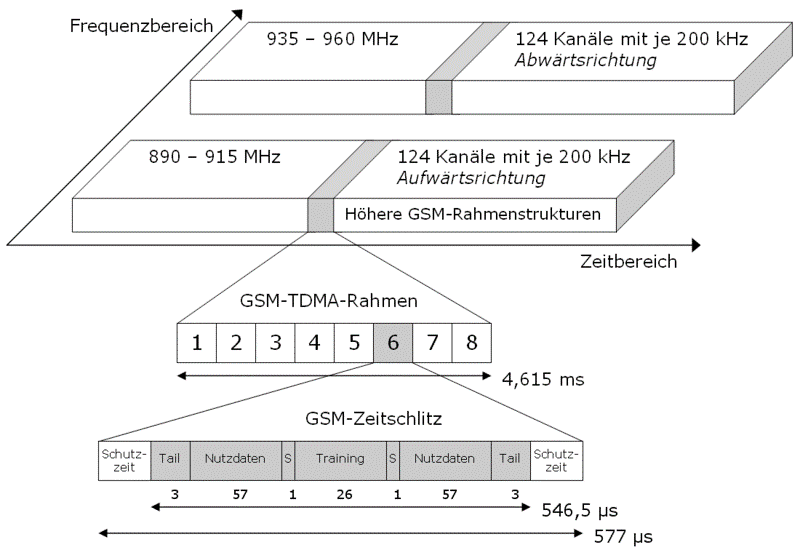
\includegraphics[width=\linewidth]{Kapitel/2G/Grafiken/GSM-Frequenzaufteilung.png}
\captionof{figure}{GSM Frequenzaufteilung~\cite{G2.3}}
\label{fig:G2.frequenzaufteilung}
\end{Figure}
\noindent
Um nun Authentifizierung, Authorisierung und eine korrekte Übertragung zu gewährleisten, werden weitere Bits abgezogen, sodass am Ende eine Datenrate von \SI{9,6}{kbit/s} erreicht wird. \cite{G2.1}\cite{G2.3}
\subsubsection*{Struktur des Mobilfunknetzes}
Aus der vorhergehenden Strukturerklärung ist zu erkennen, dass mit einem solchen System nur rund 1000 Mobilfunkgeräte gleichzeitig genutzt werden können. Dies ist für ein globales Netz aber bei weitem nicht ausreichend. Deswegen kommt nun der zelluläre Aufbau des Netzes zum Tragen, also die Technik des \textit{Raummultiplexing} (\textbf{SDMA} - \textbf{S}pace \textbf{D}ivision \textbf{M}ultiplex \textbf{A}ccess).\cite{G2.2}
\begin{Figure}
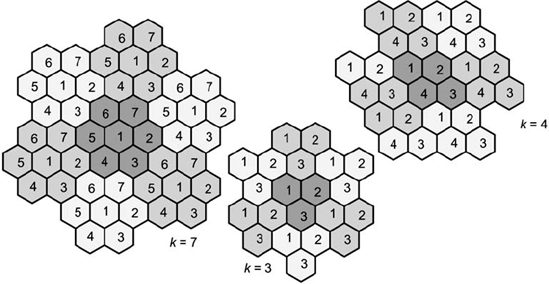
\includegraphics[width=\linewidth]{Kapitel/2G/Grafiken/GSM-Funkzellenideal.png}
\captionof{figure}{GSM Funkzellenideal~\cite{G2.2}}
\label{fig:G2.funkzellenideal}
\end{Figure}
%,height=2.5cm
%letzten beiden Sätze wirken holprig
Um SDMA anzuwenden werden die Frequenzbereiche für Up- und Downlink nochmals unterteilt, um Interferenzen zwischen den unterschiedlichen Netzzellen zu minimieren. Somit haben benachbarte Netzsegmente immer verschiedene Frequenzbereiche. Dies wird mithilfe hexagonaler Waben idealisiert dargestellt (siehe Abb. \ref{fig:G2.funkzellenideal}). In der Realität werden die Strukturen der Netzsegmente, besonders im städtischen Umfeld, durch Häuser, Straßen, Flüsse und andere Faktoren beeinflusst, weshalb von dem wabenförmigen Aufbau abgewichen werden muss (siehe Abb. \ref{fig:G2.funkzellen}).
%Dies ist natürlich eine idealisierte Darstellung, wenn eine bessere Näherung wie in Abb. \ref{fig:G2.funkzellen} aussieht, die insbesondere in städtischem Umfeld durch Häuser, Straßen, Flüsse und anderes beeinflusst wird. \cite{G2.2}
\begin{Figure}
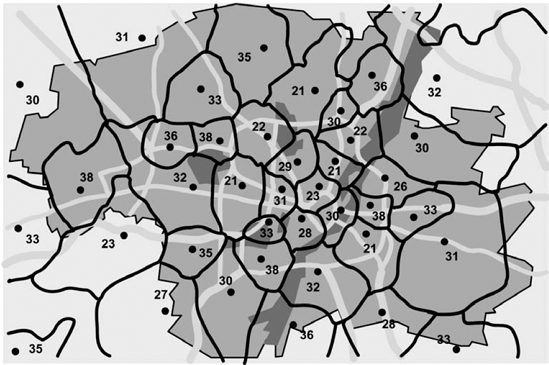
\includegraphics[width=\linewidth]{Kapitel/2G/Grafiken/GSM-Funkzellen.png}
\captionof{figure}{GSM Funkzellen~\cite{G2.2}}
\label{fig:G2.funkzellen}
\end{Figure}
%Einleitung sucked
Es folgt die nächste Überlegung, dass sich mobile Geräte in verschiedenen Zellen aufhalten, oder während eines laufenden Gesprächs von Zelle zu Zelle bewegen. Hierbei erfolgt ein \textit{Hand\-shake} zur Verbindungsübergabe, der den Übergang eines mobilen Gerätes von der aktuellen Funkzelle in die nächste Funkzelle regelt.
Vereinfacht lässt sich dies in Abb. \ref{fig:G2.handshake} beschreiben. Hierbei spricht man von dem Mobilfunkteilnehmer, der sich automatisch in die, in der Bewegungsrichtung befindenden, Basisstation einbucht, während er in der vorherigen Basistation ausgebucht wird.\cite{G2.3}
\begin{Figure}
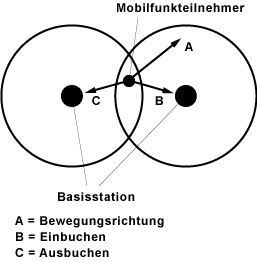
\includegraphics[width=\linewidth]{Kapitel/2G/Grafiken/GSM-Handshake.png}
\captionof{figure}{GSM Handshake~\cite{G2.2}}
\label{fig:G2.handshake}
\end{Figure}
\subsubsection*{SIM}
Das \textit{\textbf{S}ubscriber \textbf{I}dentiy \textbf{M}odule}(siehe Abb. \ref{fig:G2.sim}), kurz \textbf{SIM} oder oft SIM-Card genannt, ist ein Chip, den jedes GSM-Gerät benötigt, um sich in ein, dem GSM-Standard entsprechendes, Funk\-netz einwählen zu können. Diese SIM-Card enthält unter anderem eine \textbf{IMSI} (\textbf{I}nternational \textbf{M}obile \textbf{S}ubscriber \textbf{I}dentity). Diese maximal 15 Zeichen lange dezimale Zahl wird wie folgt aufgeteilt:
\begin{itemize}
	\item Mobile Country Code (MCC), drei Zahlen, International standardisiert (z.B. 262 für Deutschland)
	\item Mobile Network Code (MNC), zwei Zahlen, eindeutige Identifikation eines Netzanbieters des jeweiligen Landes (01, 02, 07 entsprechend für T-Mobile, Vodafone, O2)
	\item Mobile Subscriber Identification Number (MSIN), maximal 10 Zahlen, eindeutige Identifikation eines Nutzers in seinem Heimnetz
\end{itemize}
Darüber hinaus bestitzt die SIM-Card noch die Fähigkeiten PIN, Telefonbuch, Notizbuch, SMS und die zuletzt angerufenen Telefonummern und mehr zu speichern.\cite{G2.1}
\begin{Figure}
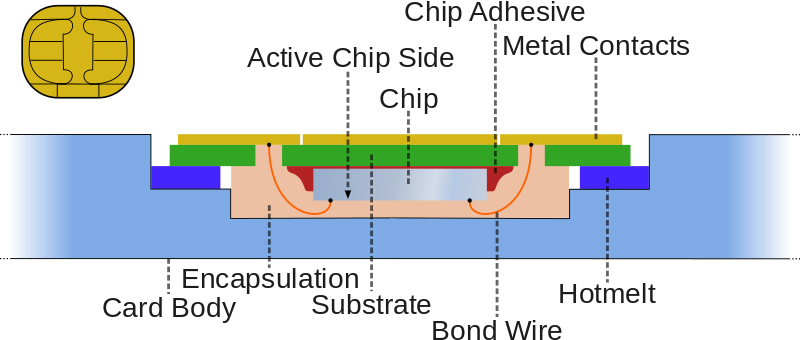
\includegraphics[width=\linewidth]{Kapitel/2G/Grafiken/GSM-SIM.png}
\captionof{figure}{GSM-SIM~\cite{G2.2}}
\label{fig:G2.sim}
\end{Figure}
%eventuell in Tabelle am Anfang reinpacken
\subsubsection*{Sonstiges}
Die Leistungsaufnahme eines solchen mobilen Geräts im 900/1800Mhz Bereich liegt bei 1/2 Watt, während eine passende Basisstation 20-50/10-20 Watt je nach Empfangsdistanz benötigt.\cite{G2.2}
\subsection*{Einsatz}
%klingt doof
Weltweit nutzen 3 Milliarden Menschen GSM als grundlegendes mobiles Kommunikationsmittel. Es ist ungewöhnlich keinen Empfang zu haben, da ein Empfang so gut wie überall möglich ist. (Siehe Abb. \ref{fig:G2.global}).
\end{multicols}
\newpage
\section*{Historische Entwicklung}
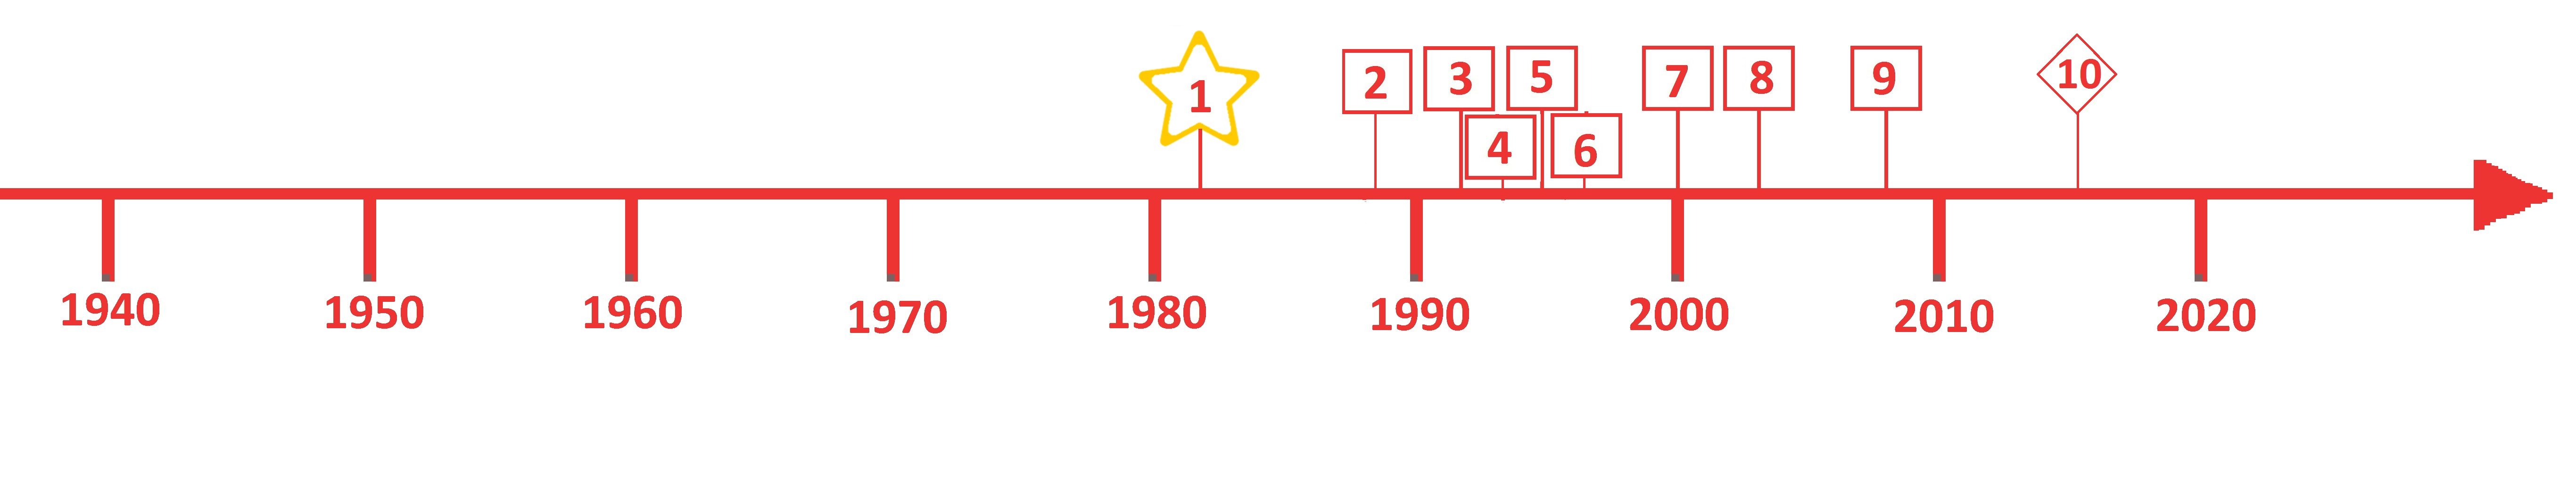
\includegraphics[width=\textwidth]{Kapitel/2G/Grafiken/Zeitstrahl}
\par
\noindent
\rowcolors{1}{\topicolor!20}{}
\begin{tabular}{p{0.5 cm}p{3 cm}p{13.55 cm}}
	Nr. & Datum & Entwicklungsschritte~ \cite{G2.1}\cite{G2.3}\\
	1 & 1982 & Die \textit{Groupe Spécial Mobile} wird eingerichtet und mit der Entwicklung eines globalen Mobilfunkstandards von der CEPT beauftragt.\\
	%CEPT kontrollieren
	2 & 1986 & Die Entscheidung für das 900Mhz Spektrum für das GSM-Band fällt.\\
	3 & 1991 & Der erste GSM-Anruf wurde in Finnland von \textit{Radiolinja} durchgeführt und leutet somit den Beginn des GSM-Mobilfunkstandards ein.\\
	4 & 1992 & Die erste SMS wird versendet.\\
	5 & 1993 & Das erste GSM-Mobiltelefon \textit{Nokia 1011} ist kommerziell erhätlich.\\
	6 & 1995 & Die Dienste über GSM angeboten werden erweitern sich um Fax, Daten und SMS Dienste.\\
	7 & 2000 & \textbf{GPRS} (\textbf{G}eneral \textbf{P}acket \textbf{R}adio \textbf{S}ervice) steht nun zur Verfügung.\\
	8 & 2003 & \textbf{EDGE} (\textbf{E}nhanced \textbf{D}ata Rates for \textbf{G}SM \textbf{E}volution) steht nun zur Verfügung.\\
	9 & 2008 & Weltweit hat der 2G-Mobilfunk mehr als drei Milliarden Nutzer.\\
	10 & 2016 & Erste Mobilfunkanbieter beginnen mit der Abschaltung von GSM-Netzen.\\
\end{tabular}
\par
\begin{multicols}{3}
%ETSI
\subsection*{Organisationen und Standardisierung}
Um ein europaweites Kommunikationsnetz zu entwickeln wurde die \textit{Groupe Spécial Mobile} von der \textbf{CEPT} (\textbf{C}onférence \textbf{E}uropéenne des Administrations des \textbf{P}ostes et des \textbf{T}élécommunications) ins Leben gerufen, die ab 1989 in der \textbf{ETSI} (\textbf{E}uropean \textbf{T}elecommunications \textbf{S}tandards \textbf{I}nstitute) aufging und das heutige Backroynm für GSM (\textbf{G}lobal \textbf{S}ystem for \textbf{M}obile Communication - \textbf{G}roupe \textbf{S}pécial \textbf{M}obile) entstanden ist. Die CEPT bietet für GSM-Operatoren ein Memorandum of Understanding an, was mit einem Standard gleichzusetzen ist, welches 2008 von 747 Mitgliedern unterschrieben wurde, die 670 GSM-Netze in 200 Ländern betreiben. \cite{G2.3}	
%wie schon erwähnt? really? Zielgruppe! 
\subsection*{Ausblick}
Wie schon erwähnt, lag die Nutzerzahl 2008 bei 3 Milliarden Nutzer. Trotzdem fangen erste Länder an G2 auszumustern. Macau ist hierbei Vorreiter, knapp gefolgt von Singapur, Australien und dem größten Mobilfunkanbieter der USA, AT\&T.
Diese Einstellung von GSM würde die Frequenzbereiche für die neueren Standards befreien, doch es gibt auch viele Netzbetreiber, insbesondere in Europa, die sich Zeit lassen, da mit Roaminggebühren, die mit GSM einhergehen, immer noch Geld verdient werden kann.\cite{G2.3}~(Bildquelle:~\cite{G2.4})
\printbibliography[segment=7,heading=subbibliography]
\end{multicols}
\begin{Figure}
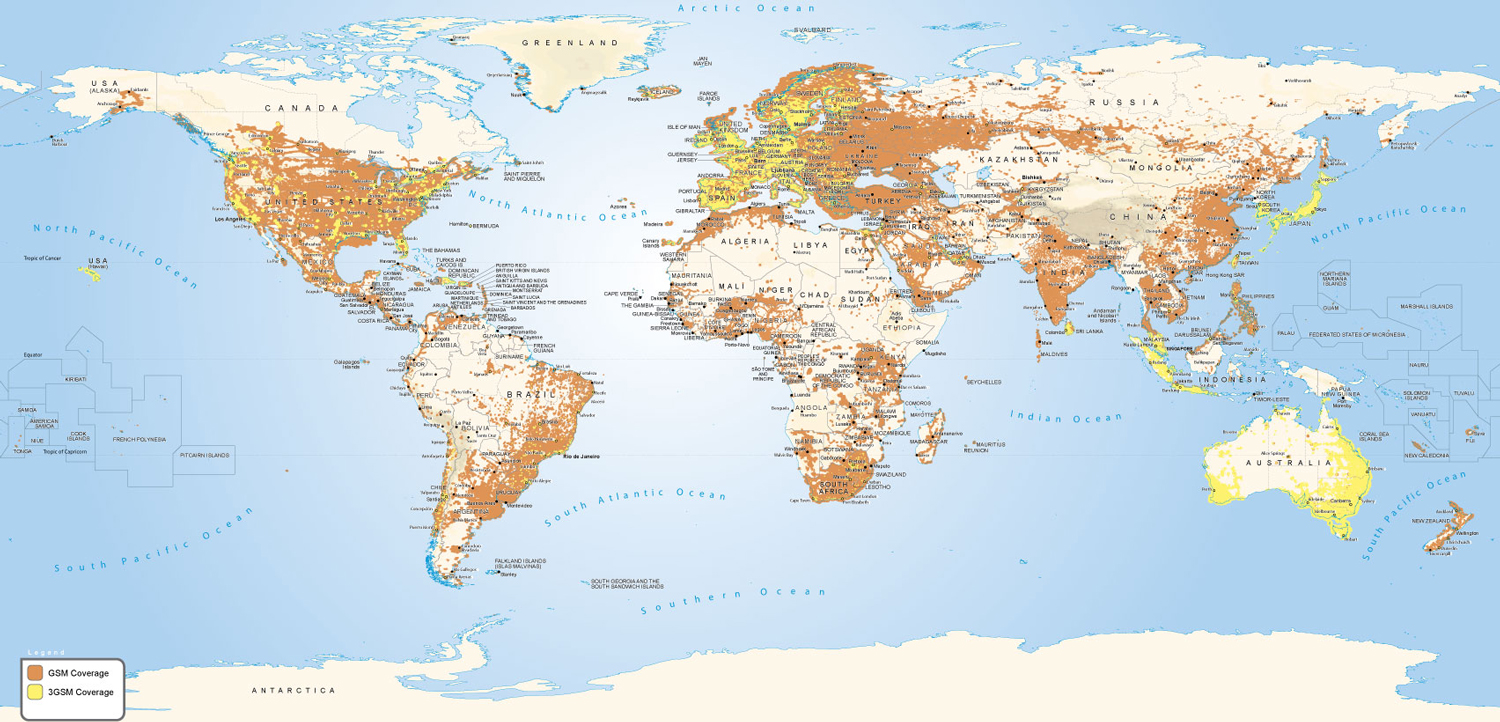
\includegraphics[width=\textwidth]{Kapitel/2G/Grafiken/GSM-Netzabdeckung-Weltweit.jpg}
\captionof{figure}{Globable Netzabdeckung (orange: GSM, gelb: UMTS)~\cite{G2.4}}
\label{fig:G2.global}
\end{Figure}
\newpage
